\documentclass{standalone}
\usepackage{tikz}
\usetikzlibrary{patterns, positioning}


\begin{document}
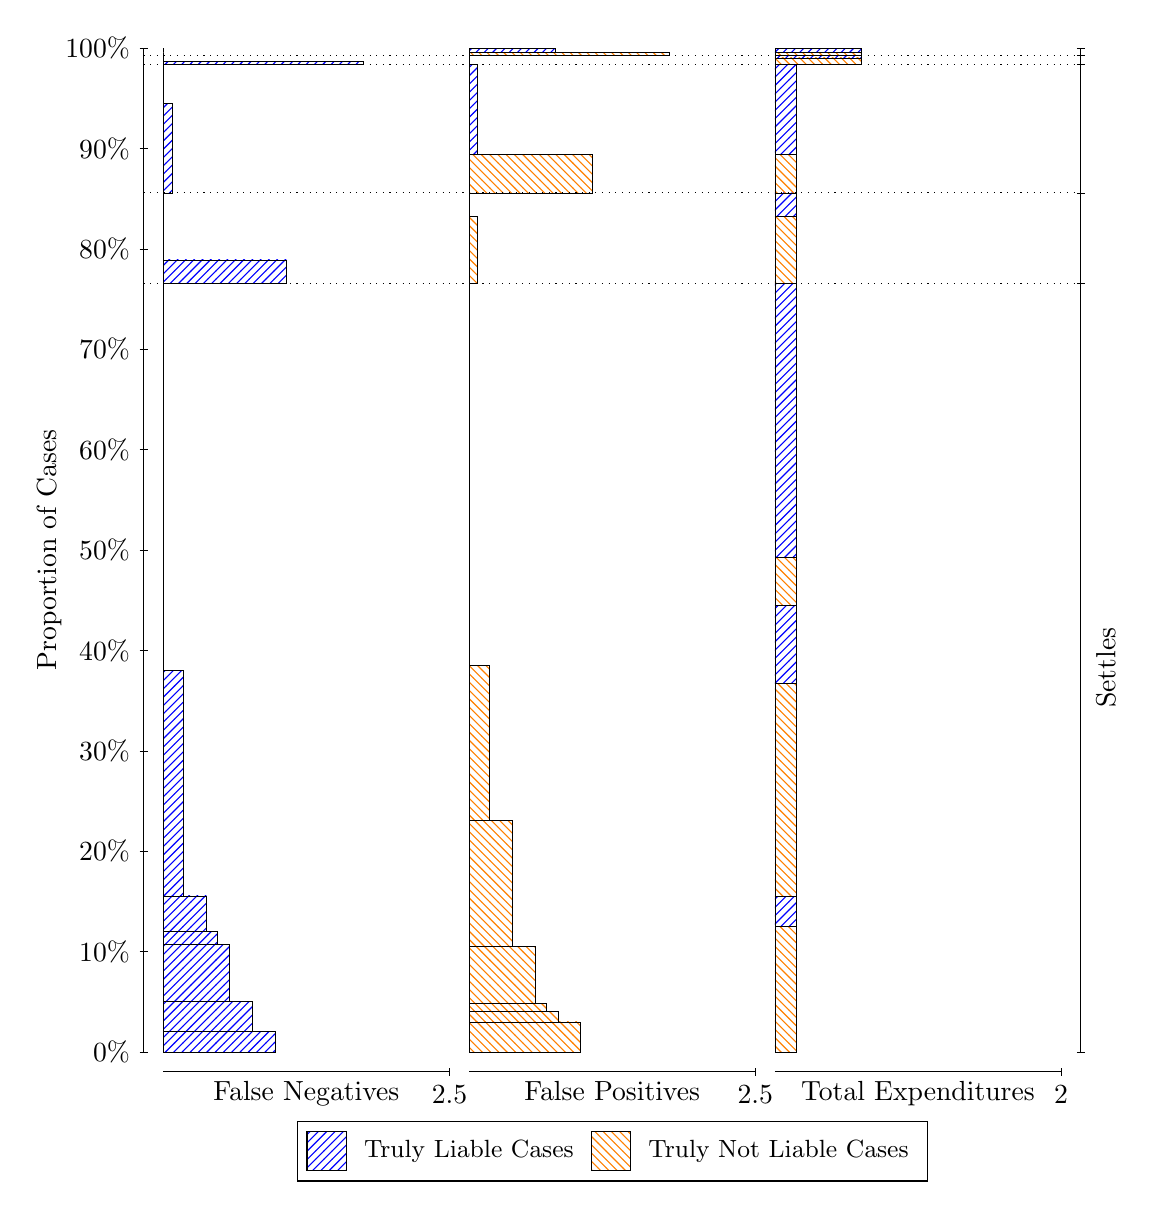
\begin{tikzpicture}
\draw[black, very thin] (1.5,1.75) -- (1.5,14.5);
\node[rotate=90, text=black, anchor=center] at (0.3, 8.125) {Proportion of Cases};
\draw[black, very thin] (1.45,1.75) -- (1.55,1.75);
\node[text=black, anchor=east] at (1.45, 1.75) {0\%};
\draw[black, very thin] (1.45,3.025) -- (1.55,3.025);
\node[text=black, anchor=east] at (1.45, 3.025) {10\%};
\draw[black, very thin] (1.45,4.3) -- (1.55,4.3);
\node[text=black, anchor=east] at (1.45, 4.3) {20\%};
\draw[black, very thin] (1.45,5.575) -- (1.55,5.575);
\node[text=black, anchor=east] at (1.45, 5.575) {30\%};
\draw[black, very thin] (1.45,6.85) -- (1.55,6.85);
\node[text=black, anchor=east] at (1.45, 6.85) {40\%};
\draw[black, very thin] (1.45,8.125) -- (1.55,8.125);
\node[text=black, anchor=east] at (1.45, 8.125) {50\%};
\draw[black, very thin] (1.45,9.4) -- (1.55,9.4);
\node[text=black, anchor=east] at (1.45, 9.4) {60\%};
\draw[black, very thin] (1.45,10.675) -- (1.55,10.675);
\node[text=black, anchor=east] at (1.45, 10.675) {70\%};
\draw[black, very thin] (1.45,11.95) -- (1.55,11.95);
\node[text=black, anchor=east] at (1.45, 11.95) {80\%};
\draw[black, very thin] (1.45,13.225) -- (1.55,13.225);
\node[text=black, anchor=east] at (1.45, 13.225) {90\%};
\draw[black, very thin] (1.45,14.5) -- (1.55,14.5);
\node[text=black, anchor=east] at (1.45, 14.5) {100\%};

\draw[black, very thin] (13.4,1.75) -- (13.4,14.5);
\draw[black, very thin] (13.35,1.75) -- (13.45,1.75);
\node[anchor=west] at (13.35, 1.75) {};
\draw[black, very thin] (13.35,11.512) -- (13.45,11.512);
\node[anchor=west] at (13.35, 11.512) {};
\draw[black, very thin] (13.35,12.661) -- (13.45,12.661);
\node[anchor=west] at (13.35, 12.661) {};
\draw[black, very thin] (13.35,14.292) -- (13.45,14.292);
\node[anchor=west] at (13.35, 14.292) {};
\draw[black, very thin] (13.35,14.409) -- (13.45,14.409);
\node[anchor=west] at (13.35, 14.409) {};
\draw[black, very thin] (13.35,14.5) -- (13.45,14.5);
\node[anchor=west] at (13.35, 14.5) {};

\draw[black, very thin, pattern color=blue, pattern=north east lines] (1.75,1.75) rectangle (3.167,2.01);
\draw[black, very thin, pattern color=blue, pattern=north east lines] (1.75,2.01) rectangle (2.8763,2.3899);
\draw[black, very thin, pattern color=blue, pattern=north east lines] (1.75,2.3899) rectangle (2.5857,3.1207);
\draw[black, very thin, pattern color=blue, pattern=north east lines] (1.75,3.1207) rectangle (2.4403,3.2819);
\draw[black, very thin, pattern color=blue, pattern=north east lines] (1.75,3.2819) rectangle (2.295,3.7331);
\draw[black, very thin, pattern color=blue, pattern=north east lines] (1.75,3.7331) rectangle (2.0043,6.5978);
\draw[black, very thin, pattern color=orange, pattern=north west lines] (1.75,6.5978) rectangle (1.75,11.512);
\draw[black, very thin, pattern color=blue, pattern=north east lines] (1.75,11.512) rectangle (3.3123,11.809);
\draw[black, very thin, pattern color=orange, pattern=north west lines] (1.75,11.809) rectangle (1.75,12.661);
\draw[black, very thin, pattern color=blue, pattern=north east lines] (1.75,12.661) rectangle (1.859,13.799);
\draw[black, very thin, pattern color=orange, pattern=north west lines] (1.75,13.799) rectangle (1.75,14.292);
\draw[black, very thin, pattern color=blue, pattern=north east lines] (1.75,14.292) rectangle (4.2933,14.326);
\draw[black, very thin, pattern color=orange, pattern=north west lines] (1.75,14.326) rectangle (1.75,14.409);
\draw[black, very thin, pattern color=orange, pattern=north west lines] (1.75,14.409) rectangle (1.75,14.443);
\draw[black, very thin, pattern color=blue, pattern=north east lines] (1.75,14.443) rectangle (1.75,14.5);
\draw[black, very thin, pattern color=orange, pattern=north west lines] (5.6333,1.75) rectangle (7.0503,2.1332);
\draw[black, very thin, pattern color=orange, pattern=north west lines] (5.6333,2.1332) rectangle (6.7597,2.2689);
\draw[black, very thin, pattern color=orange, pattern=north west lines] (5.6333,2.2689) rectangle (6.6143,2.3642);
\draw[black, very thin, pattern color=orange, pattern=north west lines] (5.6333,2.3642) rectangle (6.469,3.095);
\draw[black, very thin, pattern color=orange, pattern=north west lines] (5.6333,3.095) rectangle (6.1783,4.6892);
\draw[black, very thin, pattern color=orange, pattern=north west lines] (5.6333,4.6892) rectangle (5.8877,6.6639);
\draw[black, very thin, pattern color=blue, pattern=north east lines] (5.6333,6.6639) rectangle (5.6333,11.512);
\draw[black, very thin, pattern color=orange, pattern=north west lines] (5.6333,11.512) rectangle (5.7423,12.363);
\draw[black, very thin, pattern color=blue, pattern=north east lines] (5.6333,12.363) rectangle (5.6333,12.661);
\draw[black, very thin, pattern color=orange, pattern=north west lines] (5.6333,12.661) rectangle (7.1957,13.154);
\draw[black, very thin, pattern color=blue, pattern=north east lines] (5.6333,13.154) rectangle (5.7423,14.292);
\draw[black, very thin, pattern color=orange, pattern=north west lines] (5.6333,14.292) rectangle (5.6333,14.374);
\draw[black, very thin, pattern color=blue, pattern=north east lines] (5.6333,14.374) rectangle (5.6333,14.409);
\draw[black, very thin, pattern color=orange, pattern=north west lines] (5.6333,14.409) rectangle (8.1767,14.443);
\draw[black, very thin, pattern color=blue, pattern=north east lines] (5.6333,14.443) rectangle (6.7233,14.5);
\draw[black, very thin, pattern color=orange, pattern=north west lines] (9.5167,1.75) rectangle (9.7892,3.3442);
\draw[black, very thin, pattern color=blue, pattern=north east lines] (9.5167,3.3442) rectangle (9.7892,3.7241);
\draw[black, very thin, pattern color=orange, pattern=north west lines] (9.5167,3.7241) rectangle (9.7892,6.4295);
\draw[black, very thin, pattern color=blue, pattern=north east lines] (9.5167,6.4295) rectangle (9.7892,7.4203);
\draw[black, very thin, pattern color=orange, pattern=north west lines] (9.5167,7.4203) rectangle (9.7892,8.0346);
\draw[black, very thin, pattern color=blue, pattern=north east lines] (9.5167,8.0346) rectangle (9.7892,11.512);
\draw[black, very thin, pattern color=orange, pattern=north west lines] (9.5167,11.512) rectangle (9.7892,12.363);
\draw[black, very thin, pattern color=blue, pattern=north east lines] (9.5167,12.363) rectangle (9.7892,12.661);
\draw[black, very thin, pattern color=orange, pattern=north west lines] (9.5167,12.661) rectangle (9.7892,13.154);
\draw[black, very thin, pattern color=blue, pattern=north east lines] (9.5167,13.154) rectangle (9.7892,14.292);
\draw[black, very thin, pattern color=orange, pattern=north west lines] (9.5167,14.292) rectangle (10.607,14.374);
\draw[black, very thin, pattern color=blue, pattern=north east lines] (9.5167,14.374) rectangle (10.607,14.409);
\draw[black, very thin, pattern color=orange, pattern=north west lines] (9.5167,14.409) rectangle (10.607,14.443);
\draw[black, very thin, pattern color=blue, pattern=north east lines] (9.5167,14.443) rectangle (10.607,14.5);
\draw[black, dotted] (1.5,11.512) -- (13.4,11.512);
\draw[black, dotted] (1.5,12.661) -- (13.4,12.661);
\draw[black, dotted] (1.5,14.292) -- (13.4,14.292);
\draw[black, dotted] (1.5,14.409) -- (13.4,14.409);
\draw[black, very thin] (1.75,1.5) -- (5.3833,1.5);
\node[text=black, anchor=north] at (3.5667, 1.5) {False Negatives};
\draw[black, very thin] (5.3833,1.45) -- (5.3833,1.55);
\node[text=black, anchor=north] at (5.3833, 1.45) {2.5};

\draw[black, very thin] (5.6333,1.5) -- (9.2667,1.5);
\node[text=black, anchor=north] at (7.45, 1.5) {False Positives};
\draw[black, very thin] (9.2667,1.45) -- (9.2667,1.55);
\node[text=black, anchor=north] at (9.2667, 1.45) {2.5};

\draw[black, very thin] (9.5167,1.5) -- (13.15,1.5);
\node[text=black, anchor=north] at (11.333, 1.5) {Total Expenditures};
\draw[black, very thin] (13.15,1.45) -- (13.15,1.55);
\node[text=black, anchor=north] at (13.15, 1.45) {2};

\node[text=black, centered, rotate=90] at (13.72, 6.6308) {Settles};





\draw (7.449999999999999,1.5) node[draw=none] (baseCoordinate) {};
\begin{scope}[align=center]
        \matrix[scale=0.5, draw=black, below=0.5cm of baseCoordinate, nodes={draw}, column sep=0.1cm]{
            \node[rectangle, draw, minimum width=0.5cm, minimum height=0.5cm, pattern color=blue, pattern=north east lines] {}; &
            \node[draw=none, font=\small, text=black] (B) {Truly Liable Cases}; &
            \node[rectangle, draw, minimum width=0.5cm, minimum height=0.5cm, pattern color=orange, pattern=north west lines] {}; &
            \node[draw=none, font=\small, text=black] (B) {Truly Not Liable Cases}; \\
            };
\end{scope}

\end{tikzpicture}
\end{document}